Эксперименты ставились на парах модельных изображений и на изображениях поверхностях реальных образцов. Для тестирования использовалась следующая конфигурация.
Для корректной работы разрабатываемого программного комплекса, компьютер должен отвечать следующим требованиям:
\subsubsection {Минимальные требования к аппаратному обеспечению}
Минимальные системные требования для операционной системы Linux Debian 8~\cite{debian_8}:

\begin{itemize}
\item процессор 1ГГц Pentium 4;
\item оперативная память 512 Мб;
\item место на жёстком диске -- 9 Гб.
\end{itemize}

Минимальные системные требования для операционной системы Microsoft Windows 7~\cite{windows_7}:

\begin{itemize}
\item процессор 32-разрядный или 64-разрядный 1 ГГц;
\item оперативная память 1 Гб для 32-разрядной системы или 2 Гб для 64-разрядной системы;
\item 16 Гб для 32-разрядной системы или 20 Гб для 64-разрядной системы пространства на жестком диске;
\item графическое устройство DirectX 9 с драйвером WDDM 1.0.

\end{itemize}

\subsubsection {Минимальные требования к программному обеспечению}
Для корректной работы разрабатываемого программного комплекса на компьютере должны быть установлены:
\begin{itemize}
\item Qt5 или Qt4;
\item CMake не ниже 2.8;
\item HDF5 не ниже 1.8.
\end{itemize}
\subsection{Модельные изображения}

В качестве образцов брались наборы изображений из интернет ресурса ``Society for Experimental Mechanics (sem.org)'' описание текстур находится в таблице \ref{tab:set_image}.

\begin{longtable}[h!]{|*7{m{0.12\textwidth}|}}
\caption{Описание используемых серий изображений}
\label{tab:set_image}
\\ \hline
Серия & Имя & Метод & Диапазон яркостей 	& Уровень шума & Сдвиг (px) & Кол-во изображений \\ \hline
Grey texture & Grey set & Shift  & 0-188 & Нет & 1-20 & 5   \\ \hline
HC texture & High contrast & QEM & 10-240 & Низкий  & 0.1-1 & 122  \\ \hline
Prosilica Bin  & Sample6  & Binning & 10-156 & Низкий  & 0.1-1 & 10   \\ \hline
Strain Gradient & Sample11b & FFT & 20-185 	& Средний  & 0.01-1  & 6   \\ \hline
Strain Gradient & Sample10  & FFT & 30-225 	& Средний  & 0.01-1  & 10   \\ \hline
\end{longtable}

\subsection{Реальные отснятые изображения}

В данном разделе приведены результаты тестирования разрабатываемого программного обеспечения на изображениях поверхностей реальных образцов. В экспериментах использовались металлические образцы из авиационного алюминиевого сплава Д16АТ и полимерные образцы из полипропилена, нагружавшиеся на механической испытательной машине ИМАШ-2078 в условиях одноосного статического растяжения.

\begin{figure}[ht]
\center{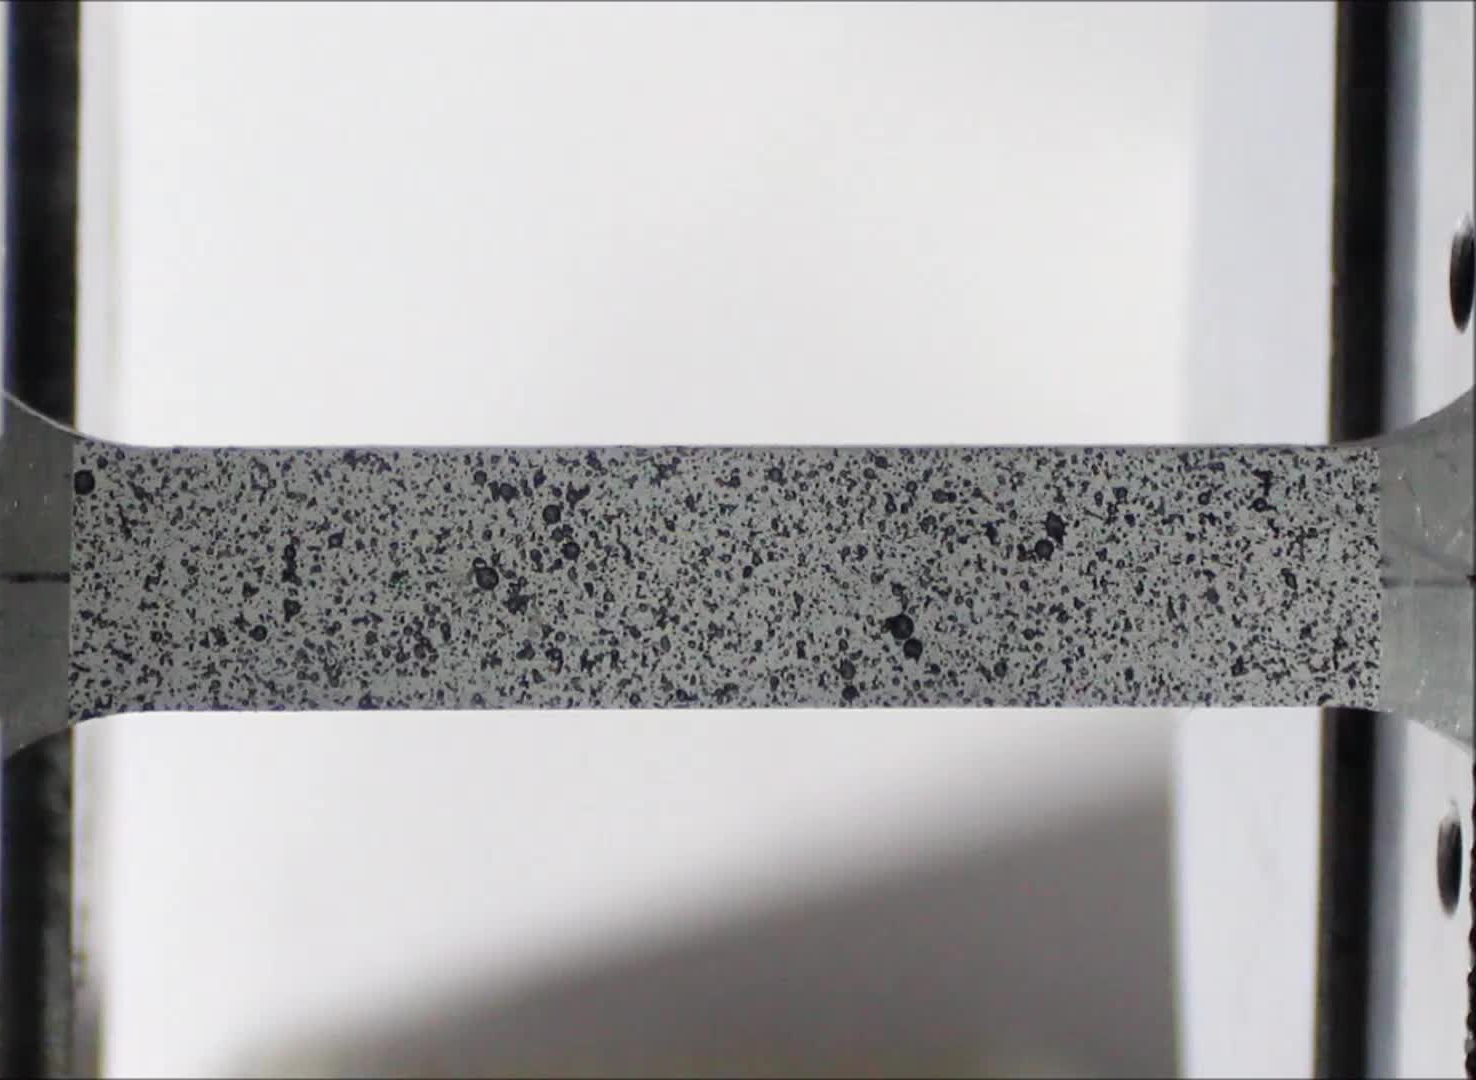
\includegraphics[width=0.6\linewidth]{real_deform}}
\caption{Растяжение пластины алюминия Д16АТ}
\label{pic:real_deform}
\end{figure}

\subsection{Тестирование на модельных изображениях}

Для первого раза используем изображения из серии Grey texture, представленные на рисунке \ref{pic:gray_set}. Они имеют сдвиг по оси $x$ на один пиксель влево, по $y$ сдвиг отсутствует.

\begin{figure}[ht]
\center{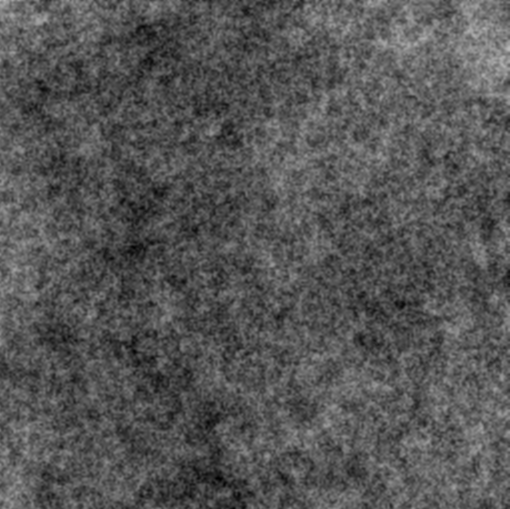
\includegraphics[width=0.6\linewidth]{gray_set}}
\caption{Тестовая серия изображений:Grey texture}
\label{pic:gray_set}
\end{figure}

Результатом работы ПО, как описано в первом разделе, является векторное поле и поля деформации твёрдого тела представленное на рисунке \ref{pic:gray_set_out}.

\begin{figure}[ht]
\center{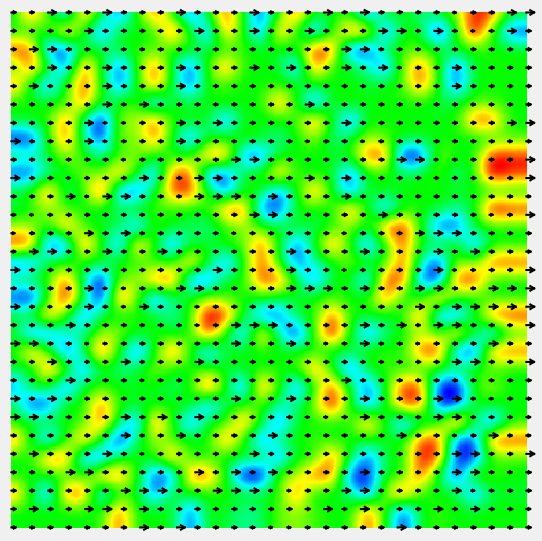
\includegraphics[width=0.6\linewidth]{gray_set_out}}
\caption{Поле смещений и деформации твёрдого тела}
\label{pic:gray_set_out}
\end{figure}

\begin{figure}[ht]
\center{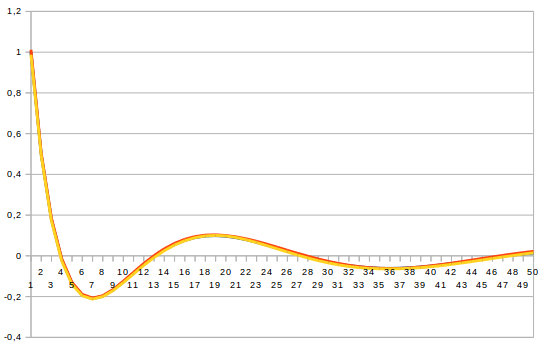
\includegraphics[width=0.6\linewidth]{gray_set_func_iteration}}
\caption{Зависимость уровня ошибки, от числа итераций}
\label{pic:gray_set_func_iteration}
\end{figure}

\begin{figure}[ht]
\center{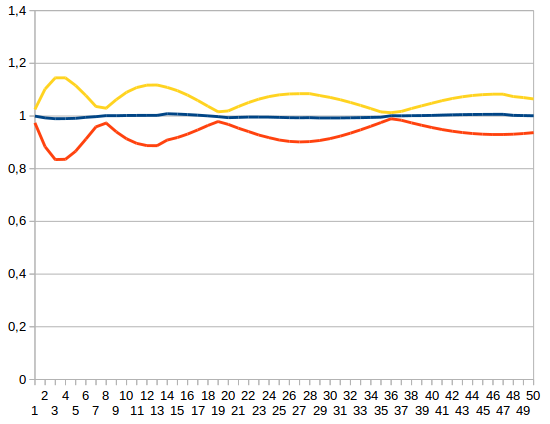
\includegraphics[width=0.6\linewidth]{gray_set_func_iter_vector}}
\caption{Зависимость смещение по x, от числа итераций}
\label{pic:gray_set_func_iter_vector}
\end{figure}

\subsection{Тестирование на экспериментально полученных изображения}